\autsection{Highly Directional Link}{Nissopoulos Ioannis}

\subsection{Link Description}

\paragraph{Directional antennas}
Directivity is a fundamental antenna parameter, which measures how much power radiated or received in a specific direction from the antenna. A directional antenna is the exact opposite of an omni-directional antenna, which transmits or receives equally from all directions. Directional antennas provide increased performance and reduced interference from unwanted sources, because of their construction and their basic principles. Well known applications for high directional antennas are among others NASA's Deep Space Network (DSN), terrestrial communication links, such as satellite television and cellular repeaters, where high position accuracy and propagation in long distances are needed. In general, high directional antennas are used in every application where high data rates, high gain and reduced interference is mandatory.

The main principle of directional antennas is their ability to concentrate almost all the transmitted power to small beamwidths, instead of illuminating wider solid angles. Saying that, they do not sacrifice any power to unwanted directions, but achieve high gain (more than 10 dBi) for specific solid angles. On the other hand, high directional antennas can reach their targets only through very narrow beamwidths, which can be a significant bottle neck in many applications and especially when tracking in long distances is required. 

Typical types of directional antennas are parabolic antennas, helical antennas, yagi antennas, horn antennas, phased arrays, etc. Directivity and gain of such types of antennas can be affected from many different parameters, regarding their type and application. The number of elements and their spacing, their physical or synthetic aperture, their surrounding environment and the manufacturing material are some of the major criterion that can change the performance of a highly directive antenna considerably. 

\paragraph{Solution description}
In this subsection we will examine if it is possible to use a high directional link for the communication segment between the lander vehicle and the penetrator of our mission. The advantages and disadvantages will be analyzed thoroughly and finally an assessment of this possibility will take place. 

The aforementioned idea is based on a pair of highly directive antennas, which can be used to achieve high rates of data streams and a stable communication channel. One antenna will be installed on lander vehicle's bottom surface looking downwards, while the other one will be placed on the top surface of the penetrator facing upwards, towards the first antenna. The line of sight between these two antennas must always be free of obstacles and we must assure that the beamwidths of the antennas are aligned and cross each other all the time. \textbf{pic} Different types of antennas will be examined in order to find out which one them is the most efficient for the requirements of our mission.

\paragraph{Drivers of Comm Link}
The design of a communication link in an inhospitable environment as Europa's subsurface can be proved especial demanding and difficult, but definitely will not be our only limitation. Space and power consumption is most of the times the number one drivers in all remotely controlled missions. The first priority when an engineer designs a communication link is the selection of the frequency range for the specific mission. In order to do so, engineers have to take into account a lot of factors such as the host environment and the attenuation that implies, the desired bandwidth, the amount of data with the corresponding data rates, etc. 

As we expect, Europa's subsurface consists of several kilometers of ice, which is a factor that limits our choice of frequency range. As described in subsection \ref{sec:ice_losses}, the longer the wavelength we use the better penetration through the ice crust we can achieve. In other words, as we go down in frequency our losses due to ice layers are diminished. Longer wavelengths are also more effective against attenuation due to impurities, because the dimensions of these impurities particles (sulfates, debris rocks, etc.) expected to be in order of millimeters. Nonetheless, the frequency of an antenna is always bonded to its size, by means that lower frequencies correspond to bigger size of antennas. Having in mind our requirements for high directivity, gain and satisfying bandwidth we must keep the size of our antenna reasonable. Other parameters that affect this size can be the type of the antenna. Moreover, due to the limited available space we will provide ways to fold and deploy the antennas wherever it is necessary.  

% \textbf{Obstacles in the near field}

\subsection{Implementation}
In this paragraph, we will examine different type of antennas for the lander vehicle, but also for the penetrating vessel. The main criteria for choosing an antenna type are the size and the ease of folding and deployment, the providing gain and the beamwidth or directivity of the antenna. Other characteristics under examination will be the capability of steering, mechanically or electronically, and the achievable data rates. After the determination of the above, we will perform the link budget analysis for the specified link. 

At first, we will concentrate only on the lander vehicle's antenna and in the next part on penetrator's. In figure \ref{fig:J_spec} can be seen the highest frequency, which is free of Jupiter's radio emissions and it is around 50 MHz, thus this is the lowest frequency choice we can make. The wavelength of this frequency is approximately 6 meters, which is way bigger than 1 meter which is the estimated available space we have under the "belly" of our land vehicle. In order to overcome this problem, we will investigate the case of a slightly higher frequencies, above 150 MHz. 

Firstly, we will present the candidate types of antennas, which will be mounted beneath our lander vehicle. It is difficult to analyze all the different types of directional antennas in the context of this report, thus we will examine three major antenna's "families", which fulfill the requirements discussed above. The first antenna type is Yagi-Uda (or Yagi) antennas together with the log periodic dipole array (LPDA). The former are used mainly from radio amateurs and they are inexpensive but quite efficient antennas for lower frequencies. A distinctive characteristic of Yagi antennas is that their design and construction based most of the times in experimental measurements hands-on experience, rather than well documented formulas and heavy mathematics. Many radio amateurs share their experience and design characteristics in order to improve the basic design as Shintaro Uda and Hidetsugu Yagi had designed in 1962. The later are a special type of antennas, which are quite similar in design with Yagis, although their distinctive characteristic is the very broad bandwidth. Because of this LPDAs are used in UHF terrestrial TV, HF communications, EMC measurements etc.

\paragraph{Yagi-Uda Design}
Yagi-Uda antennas consist of a single driven element connected to the transmitter or receiver and additional parasitic elements. The parasitic elements operate by re-radiating their signals in a slightly different phase in relation to the driven element. In this way the signal is reinforced in some directions and cancelled out in others, so a high directivity is achieved. The length and the spacing of each parasitic element determined by the operational frequency, as well as the total length of the antenna. As it can be seen in figure \ref{Yagi}, a Yagi antenna is linear polarized, parallel to its elements dimension. This is a significant drawback of this design in case the user needs to exploit different polarizations. The solution to this can be the "crossed" Yagi-Uda antenna, which practically is two antennas with two orthogonal polarizations on the same boom. Crossed Yagis provide the capability to receive or transmit in circular polarization with a -3 dB trade off of your signal. If we finally will choose this antenna type for sure we need to consider the crossed version, because the received polarization will have been rotated randomly from the ice crust. LPDAs may look similar to Yagis, although their main principle is quite different. They consist of a number of dipole elements as well, but not all antenna elements are active at any given frequency. In other words, we can imagine a LPDA as an array of dipoles tuned in different frequencies and this is the reason why these antennas hold bandwidth more than few GHz. Another difference is that the main beam of this antenna comes from the "shorter" front. LPDAs used because of their wide bandwidth and not so much because of their gain or their bandwidth. For our purposes, this antenna type will not present so many attractive points, so we will not cover them thoroughly. 

\begin{figure}[htb]
    \centering
    \begin{subfigure}[b]{0.45\textwidth}
        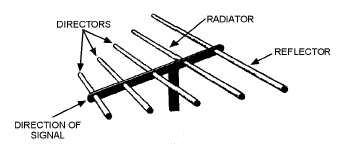
\includegraphics[width=\textwidth]{figures/Yannis/yagi.jpg}
        \caption{A typical Yagi-Uda antenna with 3 directors, 1 driven element and 1 reflectors}\label{Yagi}
    \end{subfigure}
    \begin{subfigure}[b]{0.45\textwidth}
        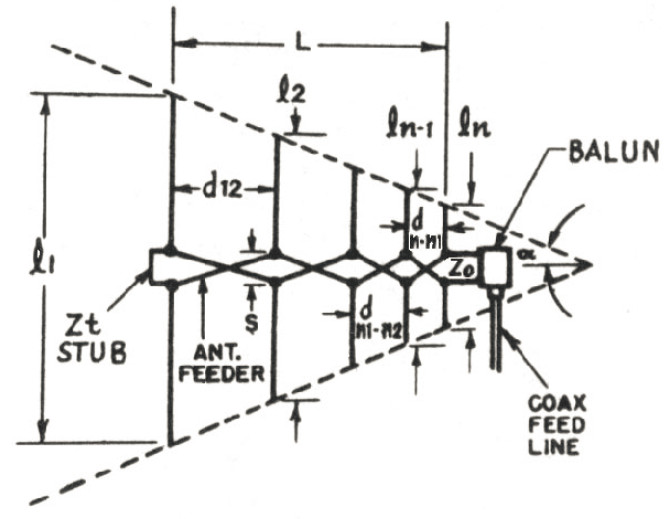
\includegraphics[width=\textwidth]{figures/Yannis/log2.jpg}
        \caption{The basic components of a log periodic dipole array. The forward direction is to the left in this sketch}\label{log}
    \end{subfigure}
    \caption{}
\end{figure}

As it is mentioned above, the design of a Yagi-Uda antenna is usually approached with an optimization algorithm based on already existed designs. Mentioning that, the free software "Yagi Calculator" (from VK5DJ radio amateur, \url{http://www.vk5dj.com/yagi.html}) was used, which simulates the antenna and has as an output its gain, beamwidth, antenna length, etc. Our major bottleneck using Yagis will be first of all their boom length. According to many designs, the boom length should be at least 2.2 $\lambda$ in order to achieve the best performance out of the antenna. Our available space is approximately 1 meter, thus our antenna boom should be less than one meter, which corresponds practically to frequencies higher than 600 MHz. As it is clear, frequencies higher than 400 MHz present excessive losses and is impossible to be used for our application. Although, we can decrease boom length according to our desires with a trade off in gain and beamwidth. Another issue that we must take into account is the really close distant of ice from the tip of our antenna. This mean that the ice will be inside the near field of our antenna, which can causes serious troubles to our design. The limit between near and far field is given by Fraunhofer's formula $d=\frac{2D^2}{\lambda}$, where D is the largest dimension of the radiator and $\lambda$ is the wavelength of the radio wave. So, we conclude that in order to eliminate or at least reduce the effect of the near field because of the ice, we have to leave a distance equals d before the ice layer. Usually, this distance is very close to the boom length, thus we could claim that we need d=80\% of boom's length, in best case scenario. 

Having the length's limitation in mind the following results came up from the software.
\begin{table}[htb]
\begin{tabular}{| c | c | c | c | c |}
\hline
 f (MHz) & Gain (dBi) & Beamwidth (-3 dB) & Boom Length (mm) & Director No. \\ 
 \hline
 300 & 8.6 & 75 & 515 & 2 \\  
 \hline
 400 & 12 & 65 & 562 & 3\\
 \hline
  430 & 11 & 57 & 700 & 4 \\
 \hline
\end{tabular}
\caption{Potential Yagi designs for different frequencies.}
\label{table: Yagi}
\end{table}

It is shown from table \ref{table: Yagi} that the beamwidths, even at 430 MHz, are fairly wide and it is difficult to define an antenna with this values as absolutely directional. Moreover, in case of a crossed design the power divided into two radiating dipoles, so we have to substract 3 dB from each case.

\paragraph{LPDA Design}
In contrast, LPDAs can be operated over a range of frequencies and over this range its electrical characteristics gain, feed-point impedance, front-to-back ratio, etc. will remain more or less constant. The two most important parameters for LPDA are $\tau$ and $\sigma$, where $\tau$ is the ratio of the length of one element to its next longest neighbor and is constant for a given design for all elements and $\sigma$ is known as the “relative spacing constant” and along with $\tau$ determines the angle of the antenna’s apex, a. 

The design process starts choosing the desired gain in dBi and from \ref{log_gain} $\tau$ and $\sigma$ are determined. A good choice of gain for this type of antennas is around 7 dBi, which is also quite common in commercial applications. Having in mind that $\tau$ and $\sigma$ define the number of elements, thus the size of antenna's boom, we want to keep them at reasonable low numbers. Observing figure \ref{log_gain}, we choose $\tau=0.9$ and $\sigma0.07$ in order to have 7 dBi gain. Also, our operational bandwidth will be from 200 to 400 MHz.

In order to find out the total length of the antenna and its number of elements the apex angle must be calculated. The bandwidth for this design is computed afterwards and from this the number of elements N and the total length of the structure are computed. Finally, the average characteristic impedance of the elements $Z_{a}$ is calculated. In the next lines these calculations take place, according to \cite{balanis}, while the MATLAB code can be found in appendix \ref{matlab}.

\begin{figure}[htb]
\centering
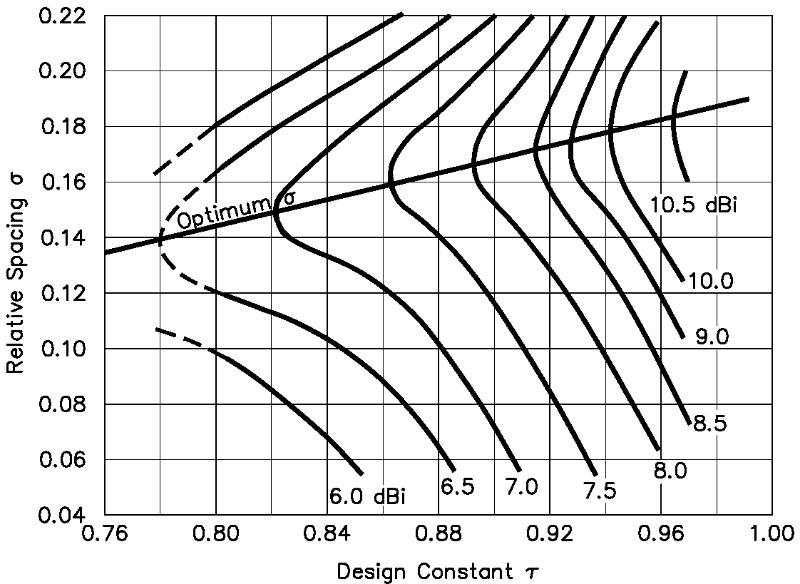
\includegraphics[width=1\textwidth]{figures/Yannis/Log_gain}
\caption{The parameters tau and sigma can be chosen from this graph. The line for optimum sigma is for those designers who want maximum gain\cite{balanis,Log}}
\label{log_gain}
\end{figure}

\begin{subequations}
\begin{align}
    a&=tan^{-1}[\frac{1-\tau}{4 \sigma}]=tan^{-1}[\frac{1-0.9}{4 \cdot 0.07}]=19.65^{\circ} \\
    B_{s}&=B \cdot B_{ar}=\frac{f_{high}}{f_{low}} (1.1+7.7(1-\tau)^2 \cdot cot(a))= \frac{400}{200} \cdot 1.316=2.631 \\
    N&=1+\frac{ln(B_{s})}{ln(\frac{1}{\tau})}=10.2 \approx 10 \ elements \\
    L&=\frac{c}{f_{low}} (1-\frac{1}{B_{s}}) \frac{cot(a)}{4}=0.6509 \ meters \\
    Z_{a}&=120(ln(\frac{l_{max}}{d})-2.25)=120 \cdot (ln(\frac{0.75}{0.019})-2.25)=171 \ \Omega
\end{align}
\label{eq: LPDA}
\end{subequations}

,where $l_{max}=\frac{c}{2 \cdot f_{min}}$ is the length of the maximum element and d=1.9 cm, which is the outer diameter of each element. Usually, a balun is needed in order to regulate the input impedance to desired values. 

LPDAs have a wide 3 dB beamwidth, which most of the times calculated through simulations, measurements or empirical tables. One f these tables is shown in figure \ref{hpbw_log}. Because of this wide beamwidth, LPDAs are not the best choice for our directional application, although if directivity is not our main concern there are manufacturers that sell very appealing, foldable antennas, some of them are presented in appendix \ref{LPDA1}. Finally, LPDAs are linear polarized, thus we have to mount two different, orthogonal antenna booms or one crossed design to receive properly the random polarization's orientation. Of course, this mean an extra 3 dB loss. A summary of the most suitable parameters of an LPDA for our mission can be found in table \ref{table: LPDA}.

\begin{figure}[htb]
\centering
    \captionsetup{width=0.8\textwidth}
        \centering
        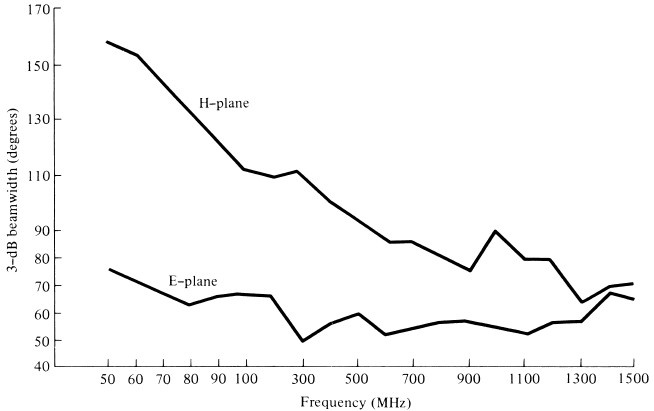
\includegraphics[width=1\textwidth]{figures/Yannis/HPBW_Log.jpg}
        \caption{Half power beamwidth for commercial log-periodic dipole arrays\cite{balanis}}
        \label{hpbw_log}
\end{figure}
\begin{figure}[htb]
\centering
        \captionsetup{width=0.8\textwidth}
        \centering
        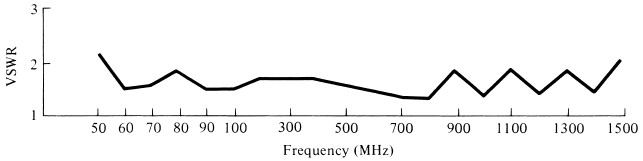
\includegraphics[width=1\linewidth]{figures/Yannis/VSWR_log.jpg}
        \caption{VSWR (Voltage Standing Wave Ratio) for commercial log-periodic dipole arrays\cite{balanis}}
        \label{vswr_lpda}
\end{figure}

\begin{table}[htb]
\begin{tabular}{| c | c | c | c | c | c | c | c |}
\hline
 $\tau$ & $\sigma$ & $f_{high}$ (MHz) & $f_{low}$ (MHz) & Gain (dBi) & HPBW & L (mm) & N \\ 
 \hline
 0.9 & 0.07 & 400 & 200 & 7 & (E)60$^\circ$-(H)100$^\circ$ & 650 & 10 \\
 \hline
\end{tabular}
\caption{Potential Log-Periodic Dipole Array design.}
\label{table: LPDA}
\end{table}

\paragraph{Helical Antennas Design}
Another type of antennas with a lot of potential in our mission is helical antenna. This antenna type is consisting of a conducting wire wound in the form of a helix, which in most cases is mounted over a ground plane. There are two modes that a helical antenna can operate and these are the normal mode and the axial. At normal mode the antenna resembles a monopole or dipole, so it has omnidirectional characteristics and linear polarization. We are interested in directional antennas, thus we will focus on the axial mode. The axial mode provides a directional antenna beam, radiating off the ends of the helix along the antenna's axis (end-fire). Moreover, the latter mode creates a circular polarized wave, which is mandatory for our application. A typical helical antenna with its radiation pattern is depicted in figure \ref{helical}.

\begin{figure}[htb]
    \centering
    \begin{subfigure}[b]{0.45\textwidth}
        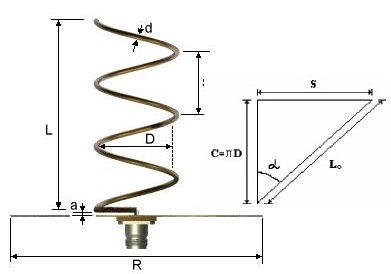
\includegraphics[width=\textwidth]{figures/Yannis/helix.jpg}
        \caption{A typical representation of a helical antenna. The most important parameters, which determine its radiation pattern are shown\cite{helix}}\label{helix1}
    \end{subfigure}
    \begin{subfigure}[b]{0.45\textwidth}
        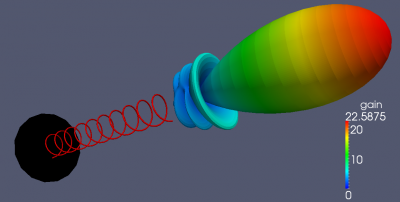
\includegraphics[width=\textwidth]{figures/Yannis/H2.png}
        \caption{Radiation pattern of helical antenna when operating in axial mode\cite{helix}}\label{helix_pat}
    \end{subfigure}
    \caption{Helical antenna sketch and radiation pattern.}\label{helical}
\end{figure}

The main constraints in building and using a helical antenna for our purposes would be again its total length, the beamwidth, the gain and the remaining distance to the ice layer. In order to examine the behaviour of such antennas the definition of the basic characteristics is needed. As it is shown in figure \ref{helix1} D represents antennas diameter, N turns of wire, d radius of wire and S the gap between turns. The overall length is $L=N \cdot S$ and the circumference of a single turn is $C=\pi \cdot D$. Last of the mechanical parameters are pitch angle of helix $a$ and R the reflector size, which must be at least 3/4 of the operating wavelength $\lambda$. In addition, we must take into account some experimentally derived guidelines, such as the value of pitch angle $a$ should be between $12^\circ$ and $14^\circ$. If $a$ is not in the specified range anomalies in the performance can occur. Also, the following formulas (eq. \ref{helical_eq}) are valid for $N \geq 3$ and $<3/4C/\lambda<4/3$ \cite{balanis2}.

For our design a trade off between total length and the parameters of frequency, C and S must be made. Generally, more turns (higher N) provide higher directivity $D_{0}$ and also the frequency dependence of the input impedance is smaller, but on the other hand the length can be disturbing big. For our mission we experimented with a MATLAB code (appendix \ref{matlab}) in different specifications and we ended up with the most suitable, as they presented in tables \ref{table: Helicals1} and \ref{table: Helicals2}. Additionally, we examined the possibility of using an array of helical antennas, but it can be seen for our frequencies it is more efficient (mainly gain-wise) to use in element. The following equations were used for this design \cite{balanis2}.

\begin{subequations}
\begin{align}
    &C=\pi \cdot D \\
    &a=tan^{-1}(\frac{S}{C}) \\
    &L=N \cdot S \\
    &R=\frac{3}{4} \lambda \\
    &Z_{in}=140 \cdot (\frac{C}{\lambda}) \\
    &HPBW=\frac{52 \cdot \lambda^{\frac{3}{2}}}{C \cdot \sqrt{N \cdot S}} \\
    &D_{0}=\frac{52 \cdot \lambda^{\frac{3}{2}}}{C \cdot \sqrt{N \cdot S}} \\
    &AR=\frac{2N+1}{2N} 
\end{align}
\label{helical_eq}
\end{subequations}

Except for a single helical antenna, we are simulated the behaviour of an array of helical antennas to examine if it is beneficial to use this implementation. The extra equations for an array are shown below (eq. \ref{helical_array}). Two approaches for the directivity were used, a simple one ($D_{array}$) and one taking into account the Hansen-Woodyard ($D_{HW}$) approximation. As it is presented in \ref{table: Helicals1} and \ref{table: Helicals2}, the array design it is not that useful for our frequencies, because in order to have better performance than the single helical antenna, more than 5 elements are needed.

\begin{subequations}
\begin{align}
    &dis=1.5 \cdot \lambda \\
    &D_{array}=N_{elem} \cdot (1+\frac{L}{dis})(\frac{dis}{\lambda}) \\
    &D_{HW}=1.805(N_{elem}(1+\frac{L}{dis})(\frac{dis}{\lambda})) 
\end{align}
\label{helical_array}
\end{subequations}
, where $N_{elem}$ is the number of array's elements and $dis$ is the distance between them. 

\begin{table}[htb]
\centering
\begin{tabular}{| c | c | c | c | c |}
\hline
 f (MHz) & Gain (dBi) & HPBW & Length (mm) & $Gain_{array}$ \\ 
 \hline
 300 & 7.8 & 64.5$^\circ$ & 800 & 16.6 \\  
 \hline
 340 & 23.6 & 37$^\circ$ & 1000 & 19\\
 \hline
  400 & 24.71 & 36.23$^\circ$ & 876 & 19.2 \\
 \hline
\end{tabular}
\caption{Helical antenna with 4 turns (N=4) specifications. The last column shows the values of gain in dBi for an array of 4 elements.}
\label{table: Helicals1}
\end{table}

\begin{table}[htb]
\centering
\begin{tabular}{| c | c | c | c | c |}
\hline
 f (MHz) & Gain (dBi) & HPBW & Length (mm) & $Gain_{array}$ \\ 
 \hline
 300 & 5.8 & 74.5$^\circ$ & 600 & 15.1 \\  
 \hline
 340 & 17.7 & 42.8$^\circ$ & 750 & 16.9\\
 \hline
  400 & 18.5 & 41.8$^\circ$ & 657 & 17.2 \\
 \hline
\end{tabular}
\caption{Helical antenna with 3 turns (N=3) specifications. The last column shows the values of gain in dBi for an array of 4 elements.}
\label{table: Helicals2}
\end{table}
A more detailed table for helical antennas can be found in appendix \ref{table: Helicals}.

As it is shown from tables \ref{table: Helicals1} and \ref{table: Helicals2}, the most suitable case is in frequency 340 MHz, where the total length of the antenna is 750 mm, the maximum gain is 17.7 dBi and the half power beamwidth is 42.8$^\circ$. There is also 250 mm free space between the end of the antenna and the ice, which could be enough to ignore ice as a near field obstacle. The gain exceeds our expectation, but bibliography states that these values may be exaggerated. But even in these case, the gain is still more than enough and helical antennas can receive or transmit circular polarization without the need of any modifications or additional losses. So, up to now it seems that a helical antenna is the most appealing option.

\paragraph{Parabolic Dish Design}
Parabolic dish antennas are very directional, high gain antennas, which are used mainly for the frequency range 2-15 GHz. For lower frequencies, like ours, the dish diameter increases to several meters. The basic formulas, which describe a dish antenna behaviour are presented below (eq. \ref{dish_eq}).

\begin{subequations}
\begin{align}
    &G=10 \cdot log_{10}(k \cdot (\pi \frac{D}{\lambda})^2) \\
    &HPBW=60 \cdot \frac{\lambda}{D}
\end{align}
\label{dish_eq}
\end{subequations}

\begin{table}[htb]
\centering
\begin{tabular}{| c | c | c | c | c |}
\hline
 f (MHz) & Gain (dBi) & HPBW & Diameter (mm) & k \\ 
 \hline
 300 & 7.2 & 66.6$^\circ$ & 900 & 0.66 \\  
 \hline
 340 & 8.3 & 58.8$^\circ$ & 900 & 0.66\\
 \hline
  400 & 9.7 & 50$^\circ$ & 900 & 0.66\\
 \hline
\end{tabular}
\caption{Parabolic antenna's specification for different frequencies.}
\label{table: dish}
\end{table}

, where G is the gain in dBi, D is the diameter of the parabolic reflector in metres and k is the efficiency factor which is generally around 50\% to 70\%. The parabolic reflector antenna gain efficiency is dependent upon a variety of factors, which are all multiplied together to give the overall efficiency. These factors are radiation efficiency, aperture taper efficiency, spillover efficiency, surface error, cross polarization, etc. The design of a parabolic antenna is way more complex, so in order to achieve very good results optimization of the feed point and a choice between different type of dish implementations must take place. By different type of dish implementations is meant, the Cassegrain, Gregorian or off-axis design. In the context of this section, we will not go any further because as it is clear from the results shown in table \ref{table: dish}, a parabolic antenna in this frequency range and under the restriction in diameter can not be really directional. Although, the gain levels are sufficient if we would like to go with a more wide HPBW.  